\documentclass{article}
\usepackage[utf8]{inputenc}
\usepackage[spanish]{babel}
\usepackage{listings}
\usepackage{graphicx}
\graphicspath{ {images/} }
\usepackage{cite}

\begin{document}

\begin{titlepage}
    \begin{center}
        \vspace*{1cm}
            
        \Huge
        \textbf{Parcial practico 1}
            
        \vspace{0.5cm}
        \LARGE
        Informe de análisis, diseño e implementación
            
        \vspace{1.5cm}
            
        \textbf{Brayan Estiben Gómez Carmona}
        
        \vspace{0.5cm}
        
        \LARGE
        \textbf{Rolman David Echavarria Prince}
        
        \vspace{0.5cm}
        
        \LARGE
        \textbf{Sebastian Zuluaga Correa}

        \vfill
            
        \vspace{0.8cm}
            
        \Large
        Despartamento de Ingeniería Electrónica y Telecomunicaciones\\
        Universidad de Antioquia\\
        Medellín\\
        Febrero de 2022
            
    \end{center}
\end{titlepage}

\tableofcontents

\newpage
\section{Objetivos}\label{intro}
Implementar un sistema de encriptación de datos que permita cifrar la información entre los sistemas de cómputo de las oficinas de una sucursal bancaria, los cuales usan infraestructura cableada para tal fin. La información viaja desde un computador de origen que es el generador de la información, hasta un computador destino que es el que se presenta al encargado de tomar decisiones en la bolsa de valores.

\subsection{Encriptación}
Desarrollar un código en la plataforma de desarrollo Qt que nos permita recibir una cadena de datos numéricos entre 0 y 255, y luego nos genere una cadena binaria correspondiente a la representación de estos datos.

\subsection{Comunicación serial}
Establecer el envío y recepción de datos entre dos dispositivos Arduino (transmisor y receptor) por medio de seis puertos digitales estableciendo una comunicación serial con dos puertos y cuatro puertos para sus respectivos relojes sincronizados.

\subsection{Paralelización de datos}
Por medio del cableado entre los Arduino conectar paralelamente un integrado 74HC595, realizar un estudio minucioso de este que nos permita obtener los datos que se envían de un Arduino hacia otro e integrar 8 datos de estos datos simultáneamente.

\subsection{Bandera}
Recibir datos generados por el integrado 74HC595 en un hardware formado por compuertas lógicas para la detección de un número en específico, que llamaremos bandera y nos servirá para dar una señal de 5 V al Arduino receptor de modo tal que se integre al código como señal de lectura.

\subsection{Desencriptación}
Desarrollar un código en nuestro Arduino receptor que nos permite clasificar por medio de unas reglas dadas la información que se requiere con base a la señal dada por medio de nuestra bandera.

\subsection{Entrega de información}
Luego de tener clasificado nuestra información, procesarla a su estado principal para entregarla a manera de visualización por medio de una pantalla LCD.

\newpage


\section{Introducción}
Se realiza un proyecto que consiste en un circuito de encriptación de la información enviada desde un PC1 con destino a un PC2, utilizando durante este proceso una combinación de hardware y software compuestos por dos dispositivos Arduino, circuito integrado 74HC545, compuertas lógicas de diferentes tipos y una pantalla LCD.\newline

En este informe se detallarán los elementos mencionados, tanto como las consideraciones, el procedimiento y la implementación del circuito final.


\newpage

\section{Marco teórico}

\subsection{Funcionamiento circuito integrado 74HC595}

\subsubsection{Descripcion}
El 74HC595 es conocido cómo registro de desplazamiento de 8 bits y sirve para expandir los puertos de un microcontrolador y también para almacenar estados lógicos, los datos ingresan de forma serial y a la salida obtenemos los datos en paralelo.\newline

Este circuito integrado consta principalmente de dos arreglos de flip-flops, el de la izquierda son 8 flip-flops encadenados en serie que permite el desplazamiento de los bits y el segundo arreglo copia los bits del primero para posteriormente mostrarlos en las salidas. \newline 

En el siguiente diagrama se pueden apreciar los dos arreglos:

\begin{figure}[!ht]
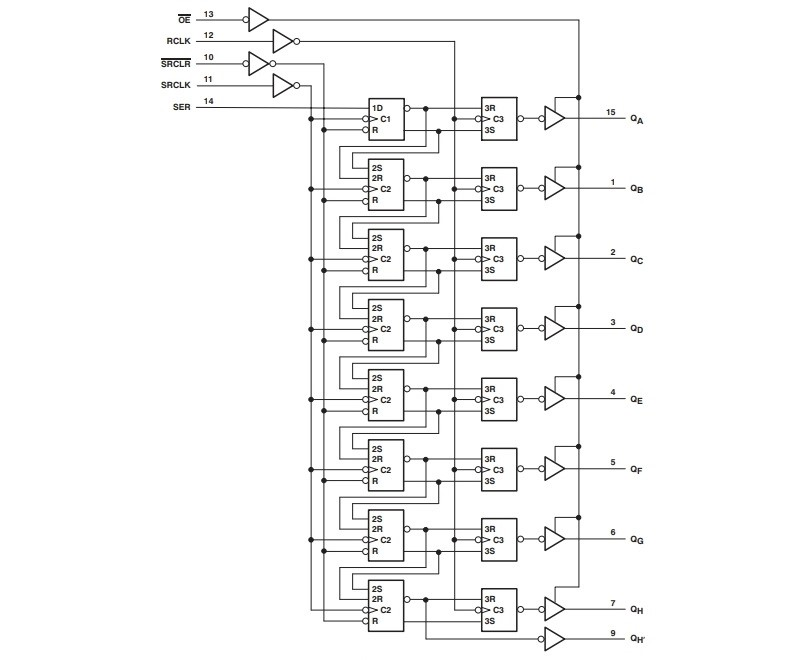
\includegraphics[width=14cm]{74HC595.jpg}
\centering
\cite{Datashet}
\end{figure}

\newpage
\begin{figure}[!ht]
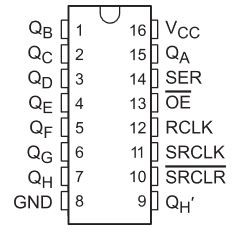
\includegraphics[width=10cm]{Pin_74HC595.jpg}
\centering
\cite{74HC595}
\end{figure}

Vamos a definir un pulso cómo el cambio de estado alto (5v) al estado bajo (0v).

\begin{figure}[!ht]
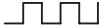
\includegraphics[width=4cm]{Pulso.jpg}
\centering
\end{figure}

Para su funcionamiento disponemos los siguientes pines:

\item
Pin 14 (SER): Este pin recibe los datos de entrada en forma serial 1 o 0.

\item
Pin 12 (RCLK): Reloj de registro de salida, en cada pulso se copia los 8 bits correspondientes de forma simultánea a un segundo conjunto de flip-flops que están conectados a las 8 salidas del circuito integrado.

\item
Pin 11 (SRCLK): Reloj de registro de desplazamiento. En cada pulso se copiará el bit que se tenga en el pin SER e irá empujando el dato al siguiente registro en serie.

\newpage

\subsubsection{Funcionamiento}
Para escribir un 0 se establece en bajo (0 voltios) el pin 14(SER) y a continuación se manda el pulso de reloj al pin 11(SRCLK), ahora el 0 está almacenado en el primer flip-flop. Si se quiere escribir un 1 entonces el pin 14(SER) se establece en alto (5 voltios) y nuevamente se manda el pulso de reloj al pin 11(SRCLK), lo que sucede es que el cero que había al inicio se desplaza al siguiente flip-flop y ahora el 1 ocupa el primero. Siguiendo esta lógica se pueden almacenar hasta 8 bits. Lo más importante es que el nuevo dato empuja a los demás una posición.\newline


Una vez se tengan los 8 bits en su posición se procede a enviar un pulso al pin 12(RCLK) copiando estos 8 bits al segundo arreglo de flip-flops de forma simultánea y así poder visualizarlos en las salidas del circuito integrado\newline. 


Es posible tener dos números diferentes dentro del IC, el registro de salida únicamente se actualiza cuando se envía un pulso de reloj al pin 12(RCLK), por lo que se puede usar para almacenar el byte bandera mientras se envían los demás bytes.\newline


 Se usará este circuito integrado para el sistema que paraleliza los datos, ya que al introducir los 8 bits en forma de serie estos son representados en cada una de las 8 salidas del chip de forma independiente. Estas 8 salidas se conectarán a la siguiente etapa que es la de desencriptación.\newline
 
 \cite{Func_integrado}

\newpage

\section{Análisis del problema}\label{intro}
Se necesita enviar información de un sistema a otro de manera encriptada de tal forma que el sistema de desencriptación esté conformado por hardware externo. Los datos deben ser enviados de modo serial, es decir, bit a bit.
Solo quienes conozcan el byte bandera pueden enviar información y que esta sea recibida de manera correcta.
El flujo de los datos es siempre del Arduino 1 hacia el Arduino.\newline




\subsection{Materiales para la implementación del sistema}

\subsubsection{Arduino 1}
Se encargará de generar la información y de enviarla

\subsubsection{Arduino 2}
Recibe la información y la procesa para ser representada de manera adecuada.

\subsubsection{74HC595}
Recibe los datos generados por el Arduino 1 a través de un puerto y paraleliza los datos que serán enviados al arreglo de compuertas.

\subsubsection{Arreglo de compuertas}
Se requiere comparar dos datos e indicarle al Arduino 2 cuál es la información que debe clasificar correctamente. En este caso se optará por el uso de solo compuertas NAND, ya que son conocidas como compuertas universales.

\subsubsection{Pantalla LCD}
Muestra el dato recibido.

\newpage
\subsection{Búsqueda información}
Para la solución se investigó sobre el funcionamiento de las compuertas lógicas y las tablas de verdad, cada uno de estos dispositivos se rigen mediante el álgebra de Boole.\newline

Se encontró un programa llamado Logisim que permite la creación de tablas de valores de forma rápida y su representación en compuertas lógicas. Además, cualquier compuerta lógica se puede representar mediante compuertas universales NAND, esto es muy útil cuando no se tienen otras compuertas deseadas para algún montaje, en este caso Tinkercad no tiene compuertas negadoras. 
\begin{figure}[!ht]
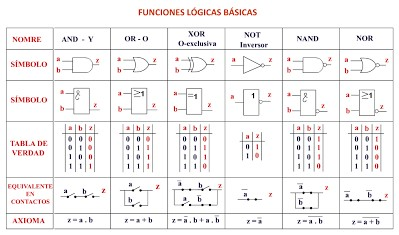
\includegraphics[width=12cm]{Funciones_logicas_basicas.jpg}
\centering
\cite{Compuertas_logicas}
\end{figure}


Al tener 8 bits se puede representar los números del 0 al 255, el sistema de desencriptación debe comparar dos números en ese rango para decidir si son iguales. El principal problema que surgió es que para comparar un número de 8 bits se requiere una gran cantidad de compuertas lógicas.


\newpage
\subsection{Procesos}

\subsubsection{Transmisión}
El PC 1 envía los datos al Arduino transmisor para generar la información a través de tres pines, uno para datos y otros dos como señal de reloj. Los datos serán enviados al circuito integrado 74HC595 de forma serial utilizando estados lógicos, 1 o 0. Los pines de reloj se usarán para controlar el registro de salida y el registro de desplazamiento del IC e ir almacenando los bits en el registro. El primer byte en el 74HC595 pasará al registro de salida mediante un pulso en el reloj de salida, se presenta el byte a la etapa de comparación que decidirá si corresponde o no al byte bandera. 

\subsubsection{Desencriptación}
Se establece un arreglo de compuertas con un byte bandera ya predefinido empleando las tablas de verdad, cómo ejemplo se toma el número 20 (00010100), con lo investigado previamente se sabe que existe un arreglo de compuertas de 8 entradas donde solo ese byte activará una salida. Si el byte que hay en las 8 salidas del 74HC595 corresponde al número 20, entonces la lógica de las compuertas activará un pulso que es enviado a una compuerta AND y esta permite el paso de los datos, en caso de que el byte no coincida con la bandera los datos que llegan al segundo Arduino son todos 0.

\subsubsection{Recepción}
En el segundo Arduino se establecen dos pines como entrada, uno de ellos para datos y el otro para la señal de reloj. Cada vez que llega un pulso de reloj el Arduino lee el dato que haya en el pin de datos. El problema es que como la señal de reloj es la misma que la del Arduino transmisor el receptor lee 8 bits que son considerados como basura mientras el byte bandera se establece en las salidas del IC 74HC595, luego el Arduino receptor continúa leyendo los otros bits del nuevo byte del arreglo, si el byte bandera es el correcto el nuevo byte se lee correctamente, en caso contrario el Arduino lee 0 en la entrada.

\subsubsection{Visualización}
Para visualizar la información se utilizará un display LCD conectado al Arduino receptor. Existen ya varios montajes de un panel LCD para el Arduino por lo que en esta etapa se buscará como adaptarlos mediante algún código que se desarrolle en C++.


\newpage

\section{Marco experimental} \label{contenido}
Aquí se estará documentando todas las acciones, procesos y demás que se estarán realizando durante la implementación del proyecto.



\newpage
\section{Conclusiones} \label{conclusiones}
En esta sección se establecerán las conclusiones finales luego de dar por terminada la implementación del proyecto.

\bibliographystyle{IEEEtran}
\bibliography{references}

\end{document}
